\chapter{प्रयोगशाला तकनीकें I: सुरक्षा, मापन और पृथक्करण}\label{ch:b1:lab-techniques-1}

दो विद्यार्थी ऐस्पिरिन के एक ही खेप का \omterm{def:b1:lab-techniques-1:recrystallisation}{पुनःक्रिस्टलन} करते हैं और उसी तप्त बेंच पर
उसका गलनांक मापते हैं। एक \qty{134}{\celsius} पढ़ता है, दूसरा
\qty{136}{\celsius}। क्या वे असहमत हैं? क्या उत्पाद शुद्ध है? किसी भी
प्रश्न का उत्तर केवल दो संख्याओं से नहीं दिया जा सकता: किसी मापन का
मूल्य केवल उसकी अनिश्चितता के साथ है, और किसी तुलना का केवल किसी
नियम के साथ। यह अंतिम अध्याय वर्ष के व्यावहारिक पक्ष को एकत्रित करता है: बेंच पर
रखी चीज़ों के \omterm{def:b1:lab-techniques-1:hazard}{संकट} कैसे पढ़े जाएँ, किसी मापे गए मान और उसकी अनिश्चितता को
कैसे व्यक्त किया जाए और उसकी तुलना किसी अन्य से कैसे की जाए, और कार्बनिक प्रयोगशाला की
पारंपरिक संक्रियाएँ --- निष्कर्षण, निस्यंदन,
\omterm{def:b1:lab-techniques-1:recrystallisation}{पुनःक्रिस्टलन}, आसवन --- किसी उत्पाद को उसके चारों ओर की चीज़ों से
कैसे पृथक करती हैं, और फिर कैसे जाँचा जाए कि वह शुद्ध है।

\begin{recall}
अंतराअणुक बलों से \omterm{def:b1:precipitation:solubility}{विलेयता} और मिश्रणीयता, ध्रुवीय और अध्रुवीय
विलायक (\cref{ch:b1:intermolecular-forces-solvents}); ब्यूरेट, पिपेट
और \omterm{def:b1:titration-methods:titration}{अनुमापन} का \omterm{def:b1:titration-methods:titration}{अंत्य बिंदु} (\cref{ch:b1:titration-methods})। विद्यालय के
खंड (कक्षा 10) ने द्रव--द्रव निष्कर्षण,
\omterm{def:b1:lab-techniques-1:recrystallisation}{पुनःक्रिस्टलन}, पतली परत वर्णलेखन और किसी संश्लेषण की \omterm{def:b1:extent-q-and-k:fractional-extent}{लब्धि} का परिचय दिया था;
यहाँ उन्हें उनकी संख्याएँ मिलती हैं।
\end{recall}

\begin{omfigure}
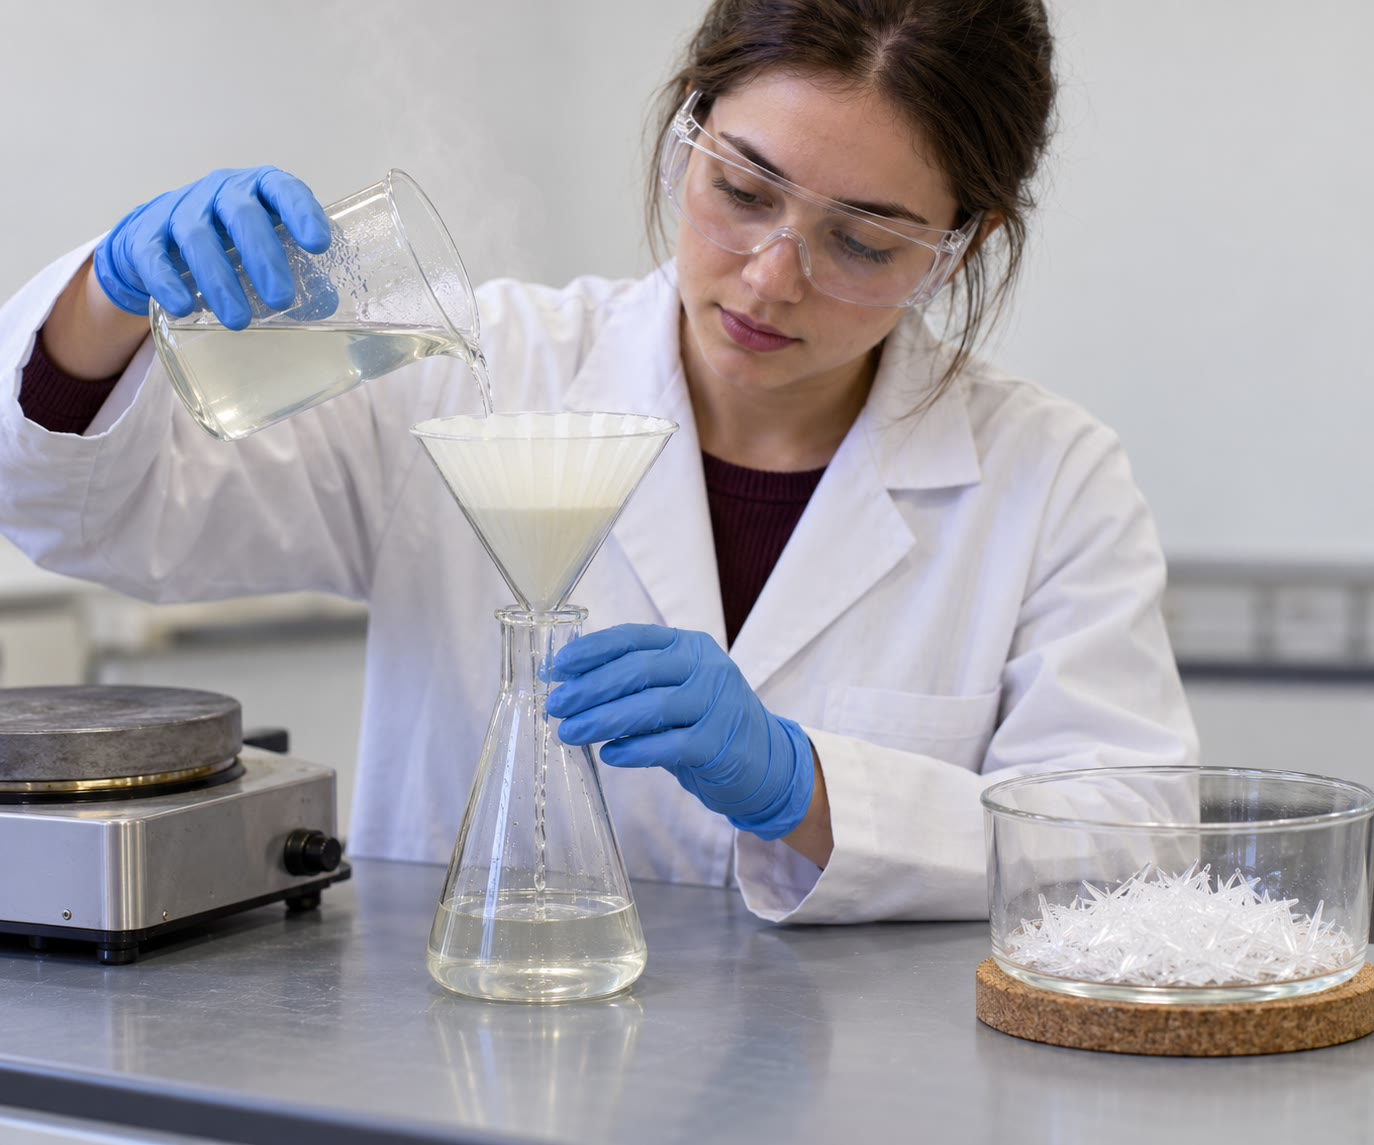
\includegraphics[width=0.5\linewidth]{images/book2/ai/b1-29-recrystallisation.jpg}

{\small \omterm{def:b1:lab-techniques-1:recrystallisation}{पुनःक्रिस्टलन} के दौरान गरम निस्यंदन: चश्मा, दस्ताने और
प्रयोगशाला कोट; गरम विलयन एक चुन्नटदार फ़िल्टर पत्र से गुज़रता है, जो
अविलेय अशुद्धियों को रोक लेता है। दाईं ओर की तश्तरी में पुनःक्रिस्टलित उत्पाद की
सुइयाँ रखी हैं।}
\end{omfigure}

\section{संकट और उनके लेबल}

\begin{definition}[संकट और जोखिम]\label{def:b1:lab-techniques-1:hazard}
\emph{संकट}\index{संकट} किसी पदार्थ (या
किसी स्थिति) का वह आंतरिक गुण है जो हानि पहुँचा सकता है: ज्वलनशीलता, संक्षारकता,
विषाक्तता। \emph{जोखिम}\index{जोखिम} इस बात की संभावना है कि हानि वास्तव में
हो, और उसकी गंभीरता, उपयोग की दी गई परिस्थितियों में: यह
संकट पर और अनावरण (मात्रा, सांद्रता, अवधि, मार्ग,
सुरक्षा उपाय) पर निर्भर करता है।
\end{definition}

पदार्थ को बदले बिना \omterm{def:b1:lab-techniques-1:hazard}{संकट} नहीं बदला जा सकता; \omterm{def:b1:lab-techniques-1:hazard}{जोखिम}
अनावरण पर काम करके घटाया जाता है: कम मात्रा, अधिक तनु
विलयन, धूम-कोष्ठ, दस्ताने और चश्मा, या उसी काम के लिए कम संकटमय अभिकर्मक।

\begin{definition}[GHS लेबलन]\label{def:b1:lab-techniques-1:ghs}
रसायनों के लेबल विश्व स्तर पर सुसंगत प्रणाली (GHS) का पालन करते हैं।
\begin{itemize}
  \item \emph{संकट चित्रलेख}\index{संकट चित्रलेख} लाल किनारे वाले
        श्वेत समचतुर्भुज पर एक काला प्रतीक है; ये नौ हैं, \texttt{GHS01}
        से \texttt{GHS09} तक।
  \item \emph{संकेत शब्द}\index{संकेत शब्द} अधिक गंभीर \omterm{def:b1:lab-techniques-1:hazard}{संकट} श्रेणियों के लिए
        \emph{ख़तरा} और कम गंभीर के लिए \emph{चेतावनी} होता है; लेबल पर
        केवल एक होता है, अधिक गंभीर वाला।
  \item \emph{संकट कथन}\index{संकट कथन} एक मानक
        वाक्यांश है, जिसका कूट H और उसके बाद तीन अंक हैं, और जो किसी \omterm{def:b1:lab-techniques-1:hazard}{संकट} का वर्णन करता है:
        H2xx भौतिक \omterm{def:b1:lab-techniques-1:hazard}{संकट}, H3xx स्वास्थ्य संकट, H4xx पर्यावरणीय
        \omterm{def:b1:lab-techniques-1:hazard}{संकट}।
  \item \emph{सावधानी कथन}\index{सावधानी कथन},
        जिसका कूट P और तीन अंक हैं, अपनाया जाने वाला उपाय बताता है: P1xx सामान्य,
        P2xx निवारण, P3xx अनुक्रिया, P4xx भंडारण, P5xx निपटान।
  \item \emph{सुरक्षा आँकड़ा पत्रक}\index{सुरक्षा आँकड़ा पत्रक} वह
        दस्तावेज़ है जो आपूर्तिकर्ता किसी उत्पाद के साथ मानक
        खंडों में देता है: पहचान, \omterm{def:b1:lab-techniques-1:hazard}{संकट}, संघटन, प्राथमिक चिकित्सा,
        अग्निशमन, संचालन और भंडारण, अनावरण नियंत्रण और
        व्यक्तिगत सुरक्षा, भौतिक और रासायनिक गुण, स्थायित्व, विषाक्तता,
        निपटान और परिवहन।
\end{itemize}
\end{definition}

\begin{omfigure}
\setlength{\tabcolsep}{5pt}
\begin{tabular}{ccccc}
\begin{tabular}[t]{@{}c@{}}\ghs[1.25cm]{GHS01}\\[2pt]\footnotesize GHS01\\\footnotesize विस्फोटक\end{tabular} &
\begin{tabular}[t]{@{}c@{}}\ghs[1.25cm]{GHS02}\\[2pt]\footnotesize GHS02\\\footnotesize ज्वलनशील\end{tabular} &
\begin{tabular}[t]{@{}c@{}}\ghs[1.25cm]{GHS03}\\[2pt]\footnotesize GHS03\\\footnotesize ऑक्सीकारक\end{tabular} &
\begin{tabular}[t]{@{}c@{}}\ghs[1.25cm]{GHS04}\\[2pt]\footnotesize GHS04\\\footnotesize दाबयुक्त गैस\end{tabular} &
\begin{tabular}[t]{@{}c@{}}\ghs[1.25cm]{GHS05}\\[2pt]\footnotesize GHS05\\\footnotesize संक्षारक\end{tabular} \\[8pt]
\begin{tabular}[t]{@{}c@{}}\ghs[1.25cm]{GHS06}\\[2pt]\footnotesize GHS06\\\footnotesize तीव्र विषाक्तता\end{tabular} &
\begin{tabular}[t]{@{}c@{}}\ghs[1.25cm]{GHS07}\\[2pt]\footnotesize GHS07\\\footnotesize हानिकारक, क्षोभक\end{tabular} &
\begin{tabular}[t]{@{}c@{}}\ghs[1.25cm]{GHS08}\\[2pt]\footnotesize GHS08\\\footnotesize स्वास्थ्य संकट\end{tabular} &
\begin{tabular}[t]{@{}c@{}}\ghs[1.25cm]{GHS09}\\[2pt]\footnotesize GHS09\\\footnotesize पर्यावरण\end{tabular} & \\
\end{tabular}

\smallskip
{\small नौ GHS चित्रलेख: फटता बम, ज्वाला, वृत्त पर ज्वाला,
गैस सिलिंडर, संक्षारण, खोपड़ी और हड्डियाँ, विस्मयादिबोधक चिह्न, स्वास्थ्य
संकट (दीर्घकालिक प्रभाव: कैंसर, उत्परिवर्तन, प्रजनन, श्वसन-मार्ग का
संवेदीकरण, श्वसन-आकांक्षा) और पर्यावरण।}
% ledger: ghspic:GHS01, ghspic:GHS02, ghspic:GHS03, ghspic:GHS04,
% ghspic:GHS05, ghspic:GHS06, ghspic:GHS07, ghspic:GHS08, ghspic:GHS09
\end{omfigure}

\begin{example}[एथेनॉल का लेबल पढ़ना]
एथेनॉल की बोतल पर चित्रलेख GHS02 और GHS07, \omterm{def:b1:lab-techniques-1:ghs}{संकेत
शब्द} \emph{ख़तरा}, और कथन H225 (अत्यंत ज्वलनशील द्रव और
वाष्प, एक भौतिक \omterm{def:b1:lab-techniques-1:hazard}{संकट}, जिसकी श्रेणी \emph{ख़तरा} की माँग करती है) और H319
(आँखों में गंभीर क्षोभ उत्पन्न करता है, एक स्वास्थ्य संकट, अकेले में \emph{चेतावनी}) होते हैं।
इसके \omterm{def:b1:lab-techniques-1:ghs}{सावधानी कथनों} में P210 (ऊष्मा, चिंगारियों और
खुली लपटों से दूर रखें; धूम्रपान निषेध), P233 (पात्र को कसकर बंद रखें), P280
(दस्ताने और नेत्र-सुरक्षा पहनें), P305+P351+P338 (आँखों में जाने पर: कई मिनट तक
जल से सावधानीपूर्वक धोएँ, कॉन्टैक्ट लेंस निकालें, धोना
जारी रखें) और P403+P235 (अच्छी तरह हवादार स्थान में भंडारित करें, ठंडा रखें) शामिल हैं।
व्यावहारिक परिणाम: जिस बेंच पर एथेनॉल प्रयुक्त हो वहाँ कोई लौ नहीं,
चश्मा, बंद बोतल।
\end{example}
% ledger: ghs:ethanol, hstat:H225, hstat:H319, pstat:P210, pstat:P233,
% pstat:P280, pstat:P305+P351+P338, pstat:P403+P235

\begin{method}[सुरक्षा आँकड़ा पत्रकों से एक सत्र की तैयारी]\label{met:b1:lab-techniques-1:read-sds}
प्रयुक्त या बनने वाले हर पदार्थ के लिए:
\begin{enumerate}
  \item उसके चित्रलेख, \omterm{def:b1:lab-techniques-1:ghs}{संकेत शब्द} और H कथन (पत्रक का खंड 2)
        पढ़िए, और भौतिक \omterm{def:b1:lab-techniques-1:hazard}{संकटों} (आग, दाब,
        अभिक्रियाशीलता) को स्वास्थ्य और पर्यावरणीय \omterm{def:b1:lab-techniques-1:hazard}{संकटों} से अलग नोट कीजिए;
  \item हर संक्रिया (तौलना, गरम करना, स्थानांतरित करना, छानना) के लिए
        अनावरण का आकलन कीजिए: मात्रा, अवस्था (वाष्पशील द्रव या
        महीन चूर्ण फेफड़ों तक पहुँचता है), अवधि;
  \item उपाय चुनिए: कम संकटमय अभिकर्मक से प्रतिस्थापन,
        छोटा पैमाना, धूम-कोष्ठ, फिर व्यक्तिगत सुरक्षा (P2xx
        कथन);
  \item किसी दुर्घटना पर अनुक्रिया (P3xx: आँखें, त्वचा, निगलना,
        आग) और हर अपशिष्ट कहाँ जाएगा (P5xx), इसकी योजना बनाइए।
\end{enumerate}
\end{method}

\begin{inthelab}[अपशिष्ट]
स्वतः कुछ भी सिंक में नहीं जाता। कार्बनिक विलायक
दो पात्रों में एकत्रित किए जाते हैं, हैलोजनित (डाइक्लोरोमेथेन, क्लोरोफ़ॉर्म) और
अहैलोजनित (एथेनॉल, प्रोपेनोन, साइक्लोहेक्सेन, एथिल एथेनोएट), क्योंकि
उनका उपचार भिन्न ढंग से होता है; जलीय अम्ल और क्षारक विलयनों को निपटान से पहले
उदासीन किया जाता है; भारी-धातु आयनों (क्रोमियम,
कॉपर, सिल्वर) के विलयनों के अपने पात्र होते हैं; टूटा काँच और संदूषित
ठोस साधारण कचरे से अलग रखे जाते हैं। लेबल पर कथन P273, ``पर्यावरण में
निर्मुक्ति से बचें'', याद दिलाता है कि प्रयोग का अंत अपशिष्ट
पात्र है, नाली नहीं।
% ledger: pstat:P273
\end{inthelab}

\section{मापन और अनिश्चितता}

कोई मापा गया मान कभी भी मापी गई राशि का यथार्थ मान नहीं होता: मापन
दोहराइए और परिणाम थोड़ा बदल जाता है; पैमाना पढ़िए और
अंतिम अंक एक अनुमान है। अनिश्चितता बताती है कि वास्तविक मान मापे गए
मान से युक्तिसंगत रूप से कितनी दूर हो सकता है।

\begin{definition}[मापन अनिश्चितता]\label{def:b1:lab-techniques-1:uncertainty}
\begin{itemize}
  \item \emph{मापन अनिश्चितता}\index{मापन अनिश्चितता}
        एक प्राचल है जो उन मानों के प्रकीर्णन का अभिलक्षण बताता है
        जो मापी गई राशि को युक्तिसंगत रूप से दिए जा सकते हैं।
  \item \emph{मानक अनिश्चितता}\index{मानक अनिश्चितता} $u(x)$
        मानक विचलन के रूप में व्यक्त वही अनिश्चितता है।
  \item \emph{A-प्रकार मूल्यांकन}\index{A-प्रकार मूल्यांकन} $u$ को
        दोहराए गए मापनों की किसी शृंखला के सांख्यिकीय विश्लेषण से प्राप्त करता है;
        \emph{B-प्रकार मूल्यांकन}\index{B-प्रकार मूल्यांकन} उसे किसी भी
        अन्य साधन से प्राप्त करता है: किसी उपकरण का अंशांकन, उसके निर्माता द्वारा बताई गई
        सहनसीमा, अंशशोधन प्रमाणपत्र, किसी सारणीबद्ध मान के अंकों
        की संख्या।
  \item \emph{विस्तारित अनिश्चितता}\index{विस्तारित अनिश्चितता}
        $U = k\,u$, मानक अनिश्चितता को एक आवरण
        गुणक $k$ से गुणा करके मिलती है, प्रायः $k = 2$; प्रसामान्य बंटन के लिए
        अंतराल $x \pm 2u$ में वास्तविक मान लगभग
        \qty{95}{\percent} प्रायिकता से होता है।
  \item \emph{आपेक्षिक अनिश्चितता}\index{आपेक्षिक अनिश्चितता}
        $u(x)/|x|$ है, जो प्रायः प्रतिशत में दी जाती है।
\end{itemize}
\end{definition}

\begin{proposition}[A-प्रकार मूल्यांकन]\label{prop:b1:lab-techniques-1:type-a}
यदि एक ही राशि के $n$ स्वतंत्र मापन $x_1, \dots, x_n$
किए जाएँ, तो सर्वोत्तम आकलन उनका माध्य $\bar x$ है; प्रायोगिक मानक
विचलन है
\[
  s = \sqrt{\frac{1}{n-1} \sum_{i=1}^{n} (x_i - \bar x)^2},
\]
और माध्य की \omterm{def:b1:lab-techniques-1:uncertainty}{मानक अनिश्चितता} $u(\bar x) = s/\sqrt{n}$ है।
\end{proposition}
\begin{proof}[\omnameProof]
\emph{इस स्तर पर स्वीकृत}; दोहराए गए मापनों की सांख्यिकी,
जिसमें $n$ छोटा होने पर प्रयुक्त स्टूडेंट गुणांक भी है,
द्वितीय वर्ष के खंड में है।
\end{proof}

\begin{omfigure}
\begin{tikzpicture}
\begin{axis}[width=7.4cm, height=5cm, xlabel={अंत्य-बिंदु आयतन (\unit{mL})},
  ylabel={पठनों की संख्या}, ymin=0, ymax=8.5, xmin=12.2, xmax=12.7,
  xtick={12.2,12.3,12.4,12.5,12.6,12.7},
  xticklabel style={/pgf/number format/fixed, /pgf/number format/precision=1},
  axis lines=left, every axis plot/.append style={line join=round}]
  \addplot[ybar, bar width=0.045, fill=omDef!35, draw=omDef!80!black]
    table[x=V, y=count] {figdata/out/bachelor-1-type-a-uncertainty-a.dat};
  \addplot[omThm, thick, smooth]
    table[x=V, y=g] {figdata/out/bachelor-1-type-a-uncertainty-b.dat};
  \draw[omProp, thick, <->] (axis cs:12.384,7.6) -- (axis cs:12.526,7.6);
  \node[omProp, font=\small, above] at (axis cs:12.455,7.6) {$\bar V \pm s$};
\end{axis}
\end{tikzpicture}\hspace{0.6cm}%
\begin{tikzpicture}
\begin{axis}[width=5.6cm, height=5cm, xlabel={$x - x_0$}, ylabel={घनत्व},
  ymin=0, ymax=0.8, xmin=-1.6, xmax=1.6, xtick={-1,0,1},
  xticklabels={$-a$, $0$, $a$}, ytick={0.5}, yticklabels={$\frac{1}{2a}$},
  axis lines=left]
  \addplot[omDef!80!black, thick, fill=omDef!25] coordinates
    {(-1,0) (-1,0.5) (1,0.5) (1,0)} \closedcycle;
  \draw[omProp, thick, <->] (axis cs:-0.577,0.62) -- (axis cs:0.577,0.62);
  \node[omProp, font=\small, above] at (axis cs:0,0.62) {$\pm a/\sqrt3$};
\end{axis}
\end{tikzpicture}

{\small बाएँ: उसी \omterm{def:b1:titration-methods:titration}{अनुमापन} \omterm{def:b1:titration-methods:titration}{अंत्य बिंदु} के बीस पठन (उदाहरणार्थ
आँकड़े), \qty{0.05}{mL} तक पढ़े गए, उसी माध्य
$\bar V = \qty{12.455}{mL}$ और मानक विचलन $s = \qty{0.071}{mL}$ वाले प्रसामान्य वक्र के साथ।
दाएँ: \omterm{def:b1:lab-techniques-1:uncertainty}{B-प्रकार मूल्यांकन} का आयताकार बंटन, ऐसा मान जिसके बारे में
केवल इतना ज्ञात है कि वह $x_0 - a$ और $x_0 + a$ के बीच है; उसका मानक विचलन
$a/\sqrt3$ है।}
\end{omfigure}

\begin{example}[बीस अंत्य बिंदु]
चित्र के बीस पठनों के लिए $\bar V = \qty{12.455}{mL}$,
$s = \qty{0.071}{mL}$ और $u(\bar V) = 0.071/\sqrt{20} = \qty{0.016}{mL}$।
एक पठन लगभग $s$ से अनिश्चित है; बीस का माध्य लगभग
$s/\sqrt{20}$ से, साढ़े चार गुना कम। परिणाम है
$V = \qty{12.46}{mL}$, $U = 2u = \qty{0.03}{mL}$ के साथ।
\end{example}

\begin{proposition}[आयताकार बंटन के लिए B-प्रकार मूल्यांकन]\label{prop:b1:lab-techniques-1:type-b}
यदि किसी राशि के बारे में केवल इतना ज्ञात हो कि वह समान
प्रायिकता से $x_0 - a$ और $x_0 + a$ के बीच कहीं भी है, तो उसकी \omterm{def:b1:lab-techniques-1:uncertainty}{मानक
अनिश्चितता} है
\[
  u = \frac{a}{\sqrt3}.
\]
\end{proposition}
\begin{proof}
प्रायिकता घनत्व $1/(2a)$ है, $[x_0 - a, x_0 + a]$ पर, और अन्यत्र
शून्य; सममिति से उसका माध्य $x_0$ है और उसका प्रसरण है
\[
  u^2 = \int_{x_0-a}^{x_0+a} (x - x_0)^2 \frac{\mathrm{d}x}{2a}
      = \frac{1}{2a} \left[\frac{t^3}{3}\right]_{-a}^{a}
      = \frac{1}{2a}\cdot\frac{2a^3}{3} = \frac{a^2}{3}. \qedhere
\]
\end{proof}

\begin{example}[एक पठन और एक सहनसीमा]
हर \qty{0.1}{mL} पर अंशांकित ब्यूरेट आधे भाग तक पढ़ी जाती है:
पठन लिखे गए मान के $\pm\qty{0.05}{mL}$ के भीतर है, इसलिए
$u = 0.05/\sqrt3 = \qty{0.029}{mL}$। \qty{20}{mL} की पिपेट, जिसका निर्माता
$\pm\qty{0.03}{mL}$ की सहनसीमा बताता है, अपना आयतन
$u = 0.03/\sqrt3 = \qty{0.017}{mL}$ के साथ देती है। \qty{135}{\celsius} के रूप में दिया गया
सारणीबद्ध मान $\pm\qty{0.5}{\celsius}$ तक ज्ञात है: $u = \qty{0.29}{\celsius}$।
\end{example}

\begin{proposition}[अनिश्चितताओं का संयोजन]\label{prop:b1:lab-techniques-1:combine}
स्वतंत्र राशियों के लिए: यदि $y = x_1 + x_2$ या $y = x_1 - x_2$, तो
$u(y)^2 = u(x_1)^2 + u(x_2)^2$; यदि $y = x_1 x_2$ या $y = x_1/x_2$, तो
\[
  \left(\frac{u(y)}{y}\right)^2 = \left(\frac{u(x_1)}{x_1}\right)^2
  + \left(\frac{u(x_2)}{x_2}\right)^2 .
\]
एक ही राशि पर अनिश्चितता के कई स्रोत (एक A-प्रकार भाग और
B-प्रकार भाग) इसी ढंग से, वर्गों के योग के रूप में, संयोजित होते हैं।
\end{proposition}
\admitted

अनिश्चितताएँ स्वयं नहीं, उनके वर्ग जुड़ते हैं: दो स्वतंत्र
त्रुटियाँ शायद ही कभी पूरे आकार में एक ही दिशा में धकेलती हैं। अनुमापित आयतन
ब्यूरेट के दो पठनों का अंतर है, इसलिए उसकी पठन अनिश्चितता
$\sqrt2 \times \qty{0.029}{mL} = \qty{0.041}{mL}$ है; और अनिश्चितता का एक बड़ा स्रोत
अन्य स्रोतों पर हावी रहता है, और सुधार वहीं खोजना
चाहिए। आंशिक अवकलजों वाला सामान्य नियम
द्वितीय वर्ष के खंड का विषय है।

\begin{method}[परिणाम प्रस्तुत करना]\label{met:b1:lab-techniques-1:report-result}
\begin{enumerate}
  \item अनिश्चितता के स्रोतों की सूची बनाइए; हर एक का \omterm{def:b1:lab-techniques-1:uncertainty}{मानक
        अनिश्चितता} के रूप में मूल्यांकन कीजिए (शृंखला से A-प्रकार, अर्ध-चौड़ाई से
        $a/\sqrt3$ के रूप में B-प्रकार)।
  \item उन्हें वर्गों के योग के रूप में संयोजित कीजिए (\cref{prop:b1:lab-techniques-1:combine})।
  \item \omterm{def:b1:lab-techniques-1:uncertainty}{विस्तारित अनिश्चितता} $U = 2u$ एक या दो
        सार्थक अंकों के साथ दीजिए, और मान को उसी दशमलव स्थान तक
        पूर्णांकित कीजिए: $x = (\text{मान} \pm U)$ इकाई, $k = 2$।
\end{enumerate}
\end{method}

\begin{definition}[प्रसामान्यीकृत विचलन]\label{def:b1:lab-techniques-1:z-score}
\emph{प्रसामान्यीकृत विचलन}\index{प्रसामान्यीकृत विचलन} (या $z$-स्कोर), एक ही राशि के
दो स्वतंत्र मानों $x_1$ और $x_2$ के बीच, जिनकी
\omterm{def:b1:lab-techniques-1:uncertainty}{मानक अनिश्चितताएँ} $u_1$ और $u_2$ हैं, यह है
\[
  z = \frac{|x_1 - x_2|}{\sqrt{u_1^2 + u_2^2}} .
\]
दोनों मान संगत कहे जाते हैं जब $z \le 2$; कोई मापा गया मान
किसी संदर्भ मान से इसी शर्त पर संगत है।
\end{definition}

\begin{example}[दो विद्यार्थी]
आरंभ के दोनों गलनांक, \qty{134}{\celsius} और
\qty{136}{\celsius}, प्रत्येक \qty{0.8}{\celsius} की \omterm{def:b1:lab-techniques-1:uncertainty}{मानक अनिश्चितता} के साथ
प्राप्त हुए थे (बेंच का पठन और अंशशोधन)। तब
$z = 2/\sqrt{0.8^2 + 0.8^2} = 1.8 \le 2$: विद्यार्थी सहमत हैं। उनका माध्य,
\qty{135}{\celsius}, ऐस्पिरिन के सारणीबद्ध गलनांक से भी संगत है,
तीव्र तापन पर \qty{135}{\celsius}। इकाई तक दिए गए सारणीबद्ध मान का
$u = 0.5/\sqrt3 = \qty{0.29}{\celsius}$ है, इसलिए $u = \qty{0.8}{\celsius}$ वाला एक अकेला
पठन उससे तब तक संगत है जब तक वह उससे
$2\sqrt{0.8^2 + 0.29^2} = \qty{1.7}{\celsius}$ के भीतर हो: लगभग \qty{133}{\celsius}
से नीचे का पठन अशुद्ध उत्पाद की ओर संकेत करता।
\end{example}
% ledger: mp:aspirin

\section{पृथक्करण}

\begin{definition}[विभाजन गुणांक]\label{def:b1:lab-techniques-1:partition-coefficient}
जब कोई विलेय A साम्यावस्था में दो अमिश्रणीय
विलायकों, एक कार्बनिक \omterm{def:b1:extent-q-and-k:system}{प्रावस्था} और एक जलीय \omterm{def:b1:extent-q-and-k:system}{प्रावस्था}, के बीच बँटा होता है, तो उसकी
सांद्रताओं का अनुपात
\[
  K = \frac{[\mathrm{A}]_{\mathrm{org}}}{[\mathrm{A}]_{\mathrm{aq}}}
\]
तनु विलयनों के लिए किसी दिए गए ताप पर एक स्थिरांक है: दोनों
विलायकों के बीच A का \emph{विभाजन गुणांक}\index{विभाजन गुणांक}।
\end{definition}

\begin{proposition}[एक से अधिक निष्कर्षण एक से बेहतर हैं]\label{prop:b1:lab-techniques-1:multiple-extractions}
जलीय विलयन के आयतन $V_a$ का $n$ बार निष्कर्षण किया जाता है, हर बार कार्बनिक
विलायक के ताज़ा आयतन $V_o$ से। जलीय \omterm{def:b1:extent-q-and-k:system}{प्रावस्था} में बचा A का
अंश है
\[
  f_n = \left(1 + K \frac{V_o}{V_a}\right)^{-n}.
\]
विलायक के निश्चित कुल आयतन के लिए, $n$ छोटे भाग
एक बड़े भाग से अधिक निष्कर्षित करते हैं।
\end{proposition}
\begin{proof}
मान लीजिए निष्कर्षण से पहले जलीय \omterm{def:b1:extent-q-and-k:system}{प्रावस्था} में A की मात्रा $m$ है, और
बाद में $m'$। साम्य पर कार्बनिक \omterm{def:b1:extent-q-and-k:system}{प्रावस्था} में $m - m'$ है, और
$K = \dfrac{(m - m')/V_o}{m'/V_a}$, इसलिए $m - m' = K\dfrac{V_o}{V_a} m'$ और
$m' = m\big/\bigl(1 + K V_o/V_a\bigr)$। हर निष्कर्षण बची हुई
मात्रा को उसी गुणक से गुणा करता है; उनमें से $n$ के बाद $f_n$, $n$-वीं
घात है। कुल आयतन $V$ को $n$ भागों $V/n$ में बाँटने पर,
$\ln f_n = -n \ln(1 + KV/(nV_a))$; चूँकि $\ln(1+t)/t$, $t$ के साथ घटता है,
$n \ln(1 + t/n)$, $n$ के साथ बढ़ता है ($t = KV/V_a > 0$ के लिए), और $f_n$
सीमा $\mathrm{e}^{-KV/V_a}$ की ओर घटता है।
\end{proof}

\begin{example}[एक भाग या तीन]
$K = 4$ वाले एक विलेय का \qty{100}{mL} जल से
\qty{60}{mL} एथिल एथेनोएट द्वारा निष्कर्षण किया जाता है। एक भाग में,
$f_1 = 1/(1 + 4 \times 0.6) = 0.29$: \qty{71}{\percent} निष्कर्षित होता है।
\qty{20}{mL} के तीन भागों में, $f_3 = (1 + 4 \times 0.2)^{-3} = 0.17$:
\qty{83}{\percent}। एथिल एथेनोएट ($\rho = \qty{0.90}{g/cm^3}$) पृथक्कारी कीप में
ऊपरी परत है; डाइक्लोरोमेथेन
($\rho = \qty{1.33}{g/cm^3}$) निचली परत होता।
\end{example}
% ledger: rho:ethyl-acetate, rho:CH2Cl2, rho:water

निस्यंदन किसी ठोस को द्रव से पृथक करता है। गुरुत्व से, कीप में
चुन्नटदार पत्र के माध्यम से, वह किसी ऐसे गरम विलयन से अविलेय अशुद्धि को रोक लेता है
जिसे रास्ते में ठंडा नहीं होना चाहिए (गरम निस्यंदन, जैसा अध्याय के आरंभ के
छायाचित्र में है)। कम दाब पर, पार्श्व-भुजा फ़्लास्क पर लगी बुकनर कीप में
(जैसी विद्यालय के खंड में खींची गई थी), वह ठोस को
जल्दी एकत्रित करता है और उसे लगभग शुष्क छोड़ता है; ठोस को फ़िल्टर पर ही
थोड़े ठंडे विलायक से धोया जाता है।

\begin{definition}[पुनःक्रिस्टलन]\label{def:b1:lab-techniques-1:recrystallisation}
\emph{पुनःक्रिस्टलन}\index{पुनःक्रिस्टलन} किसी ठोस को
ऐसे गरम विलायक की न्यूनतम मात्रा में घोलकर शुद्ध करता है जिसमें वह गरम होने पर अत्यंत विलेय
और ठंडा होने पर अल्प विलेय हो, फिर ठंडा होने पर उसे क्रिस्टलित होने देता है; अशुद्धियाँ
या तो ठंडे विलायक (मातृद्रव) में घुली रहती हैं
या, अविलेय होने पर, पहले ही गरम निस्यंदन से हटा दी जाती हैं।
\end{definition}

\begin{method}[किसी ठोस का पुनःक्रिस्टलन]\label{met:b1:lab-techniques-1:recrystallise}
\begin{enumerate}
  \item विलायक चुनिए: उत्पाद गरम में अत्यंत विलेय और ठंडे में अल्प
        विलेय, विलेय अशुद्धियाँ ठंडे में भी विलेय, उत्पाद के साथ कोई
        अभिक्रिया नहीं, क्वथनांक उत्पाद के
        गलनांक से नीचे; दो \omterm{def:b1:intermolecular-forces-solvents:miscibility}{मिश्रणीय} विलायकों (एथेनॉल और
        जल) का मिश्रण उत्पाद के अनुसार समायोजित किया जा सकता है।
  \item अपरिष्कृत ठोस को उबलते विलायक की न्यूनतम मात्रा में घोलिए, जिसे
        छोटे भागों में मिलाया जाए, और विलायक वाष्पशील या
        ज्वलनशील हो तो पश्चवाहन के अंतर्गत।
  \item यदि कोई अविलेय अशुद्धि बची हो, तो गरम में छानिए।
  \item विलयन को धीरे-धीरे ठंडा होने दीजिए, फिर बर्फ़ में: धीमा ठंडा करना
        बड़े, अधिक शुद्ध \omterm{def:b1:crystals-metals:crystal}{क्रिस्टल} देता है, जो कम मातृद्रव फँसाते हैं।
  \item कम दाब पर छानिए, थोड़े बर्फ़-ठंडे
        विलायक से धोइए, सुखाइए, तौलिए; शुद्धता की जाँच कीजिए (गलनांक, TLC)।
\end{enumerate}
\end{method}

\begin{example}[शुद्धता की कीमत]
ऐस्पिरिन जल में \qty{25}{\celsius} पर लगभग \qty{3.3}{g/L}
और \qty{37}{\celsius} पर \qty{10}{g/L} घुलती है, क्वथनांक के पास कहीं अधिक।
यदि \qty{40}{mL} मातृद्रव और \qty{10}{mL} धोवन जल
\qty{25}{\celsius} पर फ़िल्टर से निकलें, तो वे लगभग
$\qty{0.050}{L} \times \qty{3.3}{g/L} = \qty{0.17}{g}$ ऐस्पिरिन बहा ले जाते हैं, उसकी
शुद्धता चाहे जो हो। न्यूनतम से अधिक हर मिलीलीटर विलायक की कीमत \omterm{def:b1:extent-q-and-k:fractional-extent}{लब्धि} से चुकानी पड़ती है।
\end{example}
% ledger: sol:aspirin-25, sol:aspirin-37

किसी द्रव को शुद्ध किया जाता है, या स्पष्ट रूप से भिन्न क्वथनांकों वाले दो द्रवों को
पृथक किया जाता है, \emph{सरल आसवन} द्वारा: मिश्रण उबाला जाता है, अधिक
वाष्पशील घटक से समृद्ध वाष्प संघनित करके
एकत्रित की जाती है। पार्श्व-भुजा पर ताप उस वाष्प का ताप है जो
आसवित हो रही है; जब तक वह स्थिर रहे, एक शुद्ध पदार्थ आसवित हो रहा है।
निकट क्वथनांकों वाले द्रवों के लिए प्रभाजी आसवन चाहिए, फ़्लास्क और शीर्ष के बीच एक स्तंभ,
जिसका अध्ययन द्वितीय वर्ष के खंड के द्रव--वाष्प आरेखों
के साथ होता है।

\begin{omfigure}
\begin{tikzpicture}[font=\small, scale=0.95]
  \pic[transform shape] at (0,0) {heatingmantle};
  \pic[transform shape] at (0,0) {rbflask={0.45}{orange!25}};
  \foreach \x/\y in {-0.35/0.25,0.05/0.18,0.35/0.3}
    \fill[black!55] (\x,\y) circle (0.06);
  \pic[transform shape] (s) at (0,3.0) {stillhead};
  \pic[transform shape] at ($(s-top)+(0,-0.75)$) {thermometer};
  \pic[transform shape, rotate=-20] (c) at (s-arm) {liebig={3.4}};
  \coordinate (cend) at ($(s-arm)+(-20:3.4)$);
  \pic[transform shape] (a) at (cend) {adapter};
  \pic[transform shape] at ($(a-tip)+(0,-2.4)$) {erlenmeyer={0.22}{orange!12}};
  \draw[<-, omProp, thick] (0.12,3.72) -- (-1.4,4.4) node[left, text=black,
    align=right] {तापमापी का बल्ब\\ पार्श्व-भुजा के स्तर पर};
  \draw[<-, omProp, thick] ($(s-arm)+(-20:0.65)+(0.65,0.65)$) -- ++(0.2,0.9)
    node[above, text=black] {जल बाहर};
  \draw[<-, omProp, thick] ($(s-arm)+(-20:2.7)+(-0.2,-0.6)$) -- ++(0.05,-0.9)
    node[below, text=black] {जल अंदर};
  \draw[<-, omProp, thick] (-0.3,0.27) -- (-2.2,0.7) node[left, text=black]
    {क्वथन-पत्थर};
  \draw[<-, omProp, thick] (1.35,-0.6) -- (2.3,-1.1) node[right, text=black]
    {तापन आवरण};
  \draw[<-, omProp, thick] ($(a-tip)+(0.75,-2.0)$) -- ++(1.0,0.2)
    node[right, text=black] {आसुत};
\end{tikzpicture}

{\small सरल आसवन। तापमापी संघनित्र में प्रवेश करती
वाष्प का ताप पढ़ता है; ठंडा करने वाला जल संघनित्र के निचले सिरे पर प्रवेश करता है
ताकि आवरण भरा रहे; क्वथन-पत्थर प्रचंड
उछाल को रोकते हैं; उपकरण संग्राहक पर वायु के लिए खुला है।}
\end{omfigure}

\begin{safety}{\ghs[5mm]{GHS02}}
आसवन उपकरण कभी बंद नहीं होता: गरम करने पर बंद निकाय फट जाता है।
क्वथन-पत्थर ठंडे द्रव में डाले जाते हैं, पहले से गरम द्रव में कभी
नहीं (वह तुरंत उफन सकता है)। ज्वलनशील आसुत को किसी भी लौ से
दूर एकत्रित किया जाता है, आवश्यकता हो तो संग्राहक बर्फ़ में रखकर।
\end{safety}

\section{पहचान और शुद्धता की जाँच}

\begin{definition}[मंदन गुणांक]\label{def:b1:lab-techniques-1:retention-factor}
पतली परत वर्णलेखन (TLC) में नमूने का एक धब्बा
स्थिर \omterm{def:b1:extent-q-and-k:system}{प्रावस्था} (सिलिका) से लेपित प्लेट के आधार के पास एक आधार-रेखा पर
रखा जाता है; प्लेट एक बंद टंकी में थोड़े निक्षालक में खड़ी की जाती है, जो
केशिकत्व द्वारा लेप में ऊपर चढ़ता है और स्पीशीज़ को
भिन्न दरों से ले जाता है। किसी स्पीशीज़ का \emph{मंदन गुणांक}\index{मंदन गुणांक}
है
\[
  R_f = \frac{\text{धब्बे द्वारा तय की गई दूरी}}
             {\text{निक्षालक अग्र द्वारा तय की गई दूरी}},
\]
दोनों आधार-रेखा से मापी जाती हैं; $0 \le R_f \le 1$, और दी गई
स्थिर \omterm{def:b1:extent-q-and-k:system}{प्रावस्था}, निक्षालक और ताप के लिए यह स्पीशीज़ का अभिलक्षण है।
\end{definition}

ध्रुवीय सिलिका पर, ध्रुवीय स्पीशीज़ कम
ध्रुवीय स्पीशीज़ की तुलना में अधिक प्रबलता से रोकी जाती है और उसका $R_f$ छोटा होता है; अधिक ध्रुवीय निक्षालक हर धब्बे को
और आगे ले जाता है। एक ही प्लेट पर समान $R_f$ वाली दो स्पीशीज़ फिर भी भिन्न हो सकती हैं;
दो भिन्न $R_f$ उन्हें भिन्न सिद्ध करते हैं। शुद्ध उत्पाद एक ही
धब्बा देता है।

\begin{omfigure}
\begin{tikzpicture}[font=\small, scale=1.7]
  \pic[transform shape] at (0,0) {tlcplate};
  \draw[omDef!80!black, densely dashed, line width=0.5pt] (-0.7,2.7) -- (0.7,2.7);
  \foreach \x in {-0.4,0,0.4} \fill[black!60] (\x,0.4) circle (0.025);
  \fill[omThm!70] (-0.4,{0.4+0.30*2.3}) ellipse (0.09 and 0.06);
  \fill[omDef!70] (0,{0.4+0.65*2.3}) ellipse (0.09 and 0.06);
  \fill[omThm!70] (0.4,{0.4+0.30*2.3}) ellipse (0.09 and 0.06);
  \fill[omDef!70] (0.4,{0.4+0.65*2.3}) ellipse (0.09 and 0.06);
  \node[below] at (-0.4,0) {A}; \node[below] at (0,0) {B};
  \node[below] at (0.4,0) {M};
  \draw[omProp, thick, |<->|] (0.95,0.4) -- (0.95,{0.4+0.65*2.3})
    node[midway, right] {$d_{\mathrm{B}}$};
  \draw[omProp, thick, |<->|] (1.55,0.4) -- (1.55,2.7)
    node[midway, right] {$d_{\mathrm{front}}$};
  \draw[omProp, thick, |<->|] (-0.95,0.4) -- (-0.95,{0.4+0.30*2.3})
    node[midway, left] {$d_{\mathrm{A}}$};
  \node[right, align=left, font=\footnotesize] at (0.75,2.85) {निक्षालक अग्र};
  \draw[omProp, thick, <-] (-0.6,0.4) -- (-1.2,0.05) node[left, text=black, font=\footnotesize] {आधार-रेखा};
\end{tikzpicture}

{\small एक विकसित TLC प्लेट: संदर्भ A और B तथा एक मिश्रण M,
आधार-रेखा पर रखे गए। $R_f(\mathrm{A}) = d_{\mathrm{A}}/d_{\mathrm{front}}
= 0.30$, $R_f(\mathrm{B}) = 0.65$; मिश्रण दोनों धब्बे, उन्हीं
ऊँचाइयों पर, दर्शाता है।}
\end{omfigure}

\begin{method}[TLC चलाना]\label{met:b1:lab-techniques-1:tlc}
\begin{enumerate}
  \item आधार से लगभग \qty{1}{cm} पर पेंसिल से आधार-रेखा खींचिए; नमूने और
        संदर्भों के तनु विलयनों के छोटे धब्बे
        एक-दूसरे के बगल में रखिए।
  \item टंकी में कुछ मिलीमीटर निक्षालक डालिए (आधार-रेखा से नीचे),
        उसे बंद कीजिए, वातावरण को संतृप्त होने दीजिए; प्लेट उसमें खड़ी कीजिए।
  \item जब अग्र शीर्ष से लगभग \qty{1}{cm} रह जाए तब प्लेट निकालिए;
        तुरंत अग्र चिह्नित कीजिए; सुखाइए।
  \item रंगहीन धब्बों को प्रकट कीजिए (प्रतिदीप्त प्लेट पर पराबैंगनी लैंप,
        आयोडीन वाष्प, कोई अभिरंजक); उन्हें पेंसिल से घेरिए।
  \item आधार-रेखा से दूरियाँ मापिए और हर $R_f$ परिकलित कीजिए;
        उसी प्लेट पर नमूने की तुलना संदर्भों से कीजिए।
\end{enumerate}
\end{method}

\begin{omfigure}
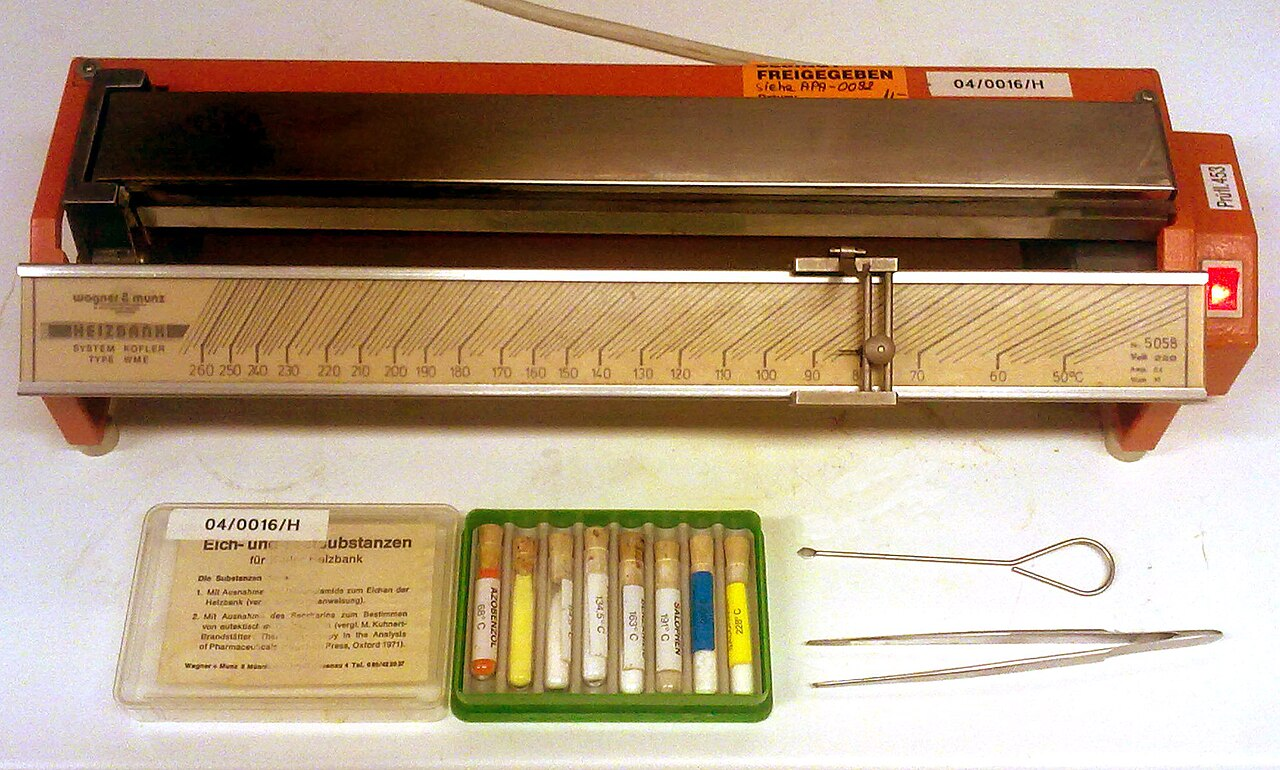
\includegraphics[width=0.62\linewidth]{images/book2/kofler-bench.jpg}

{\small एक तप्त बेंच (कोफ़्लर बेंच): एक सिरे पर गरम की गई धातु की पट्टी,
जिसकी लंबाई के साथ ताप-प्रवणता है; पट्टी पर छिड़का गया ठोस
एक तीक्ष्ण रेखा के आगे पिघलता है, जिसे सूचक से पैमाने पर पढ़ा जाता है। डिब्बे में
ज्ञात गलनांक वाले संदर्भ पदार्थ हैं, जिनसे उसका अंशशोधन किया जाता है।
छायाचित्र: एचबीआर, CC BY-SA 3.0, विकिमीडिया कॉमन्स।}
\end{omfigure}

\begin{method}[तप्त बेंच पर गलनांक मापना]\label{met:b1:lab-techniques-1:melting-point}
\begin{enumerate}
  \item बेंच को काफ़ी पहले चालू कीजिए: प्रवणता को स्थिर होने में
        समय लगता है।
  \item अपेक्षित मान के निकट पिघलने वाले किसी शुद्ध संदर्भ पदार्थ से, जिसे
        पट्टी पर छिड़का गया हो, उसका अंशशोधन कीजिए; सूचक को इस प्रकार समायोजित कीजिए कि
        रेखा पर पैमाना उसका गलनांक पढ़े।
  \item शुष्क नमूने के कुछ \omterm{def:b1:crystals-metals:crystal}{क्रिस्टल} ठंडे सिरे से
        गरम सिरे की ओर छिड़किए; उन्हें स्पैचुला से आगे-पीछे धकेलिए और
        सूचक को उस सीमा पर रखिए जिसके आगे ठोस तुरंत पिघल जाता है।
  \item पढ़िए, दोहराइए, पट्टी साफ़ कीजिए; पठनों का माध्य लीजिए और
        अनिश्चितता बताइए (\cref{met:b1:lab-techniques-1:report-result})।
\end{enumerate}
\end{method}

शुद्ध क्रिस्टलीय पदार्थ अपने गलनांक पर तीक्ष्णता से पिघलता है; अशुद्ध
पदार्थ नीचे पिघलना आरंभ करता है और एक ताप-परास में पिघलता है, क्योंकि
अशुद्धि उस ताप को घटा देती है जिस पर ठोस और द्रव
सह-अस्तित्व में रहते हैं (इसका कारण, विलेय द्वारा घटाया गया विलायक का रासायनिक विभव,
द्वितीय वर्ष के खंड में है)। सारणीबद्ध मान से काफ़ी नीचे का गलनांक,
या चौड़ा गलन-परास, इसलिए अशुद्धियों को प्रकट करता है;
\omterm{def:b1:lab-techniques-1:z-score}{प्रसामान्यीकृत विचलन} के अर्थ में सारणीबद्ध मान से संगत मान
शुद्धता का समर्थन करता है, उसे सिद्ध नहीं करता।

\begin{inthelab}[बेंच का अंशशोधन]
संदर्भों को इस प्रकार चुना जाता है कि वे अपेक्षित मान को दोनों ओर से घेरें। ऐसीटैनिलाइड,
जो \qty{114.3}{\celsius} पर पिघलता है, और बेंज़ोइक अम्ल,
\qty{122.4}{\celsius} पर, \qty{110}{\celsius} और \qty{130}{\celsius} के बीच पिघलने वाले
उत्पादों के लिए पारंपरिक मानक हैं; ऐस्पिरिन के लिए
\qty{135}{\celsius} के पास का मानक और भी बेहतर है। ऐस्पिरिन स्वयं पिघलते समय अपघटित होती है,
इसलिए उसका प्रेक्षित गलनांक इस पर निर्भर करता है कि उसे कितनी तेज़ी से गरम किया जाता है: सारणियाँ
तीव्र तापन के लिए \qty{135}{\celsius} देती हैं, और बेंच यही करती है।
% ledger: mp:acetanilide, mp:benzoic, mp:aspirin
\end{inthelab}

किसी द्रव की पहचान, और उसकी शुद्धता की जाँच, उसके \emph{अपवर्तनांक}
$n_D$ से की जाती है, जो निर्वात में प्रकाश की चाल और द्रव में उसकी चाल का
अनुपात है, जिसे सोडियम की पीली D रेखा से किसी निर्दिष्ट ताप
(प्रायः \qty{20}{\celsius}) पर, चार दशमलव स्थानों तक मापा जाता है। \qty{20}{\celsius} पर जल का
$n_D = 1.333$, एथेनॉल का 1.3611 और साइक्लोहेक्सेन का 1.4266 है।
ताप बढ़ने पर अपवर्तनांक थोड़ा घटता है, इसलिए उपकरण का
ताप स्थिर रखा जाता है।
% ledger: nD:water, nD:ethanol, nD:cyclohexane

\begin{omfigure}
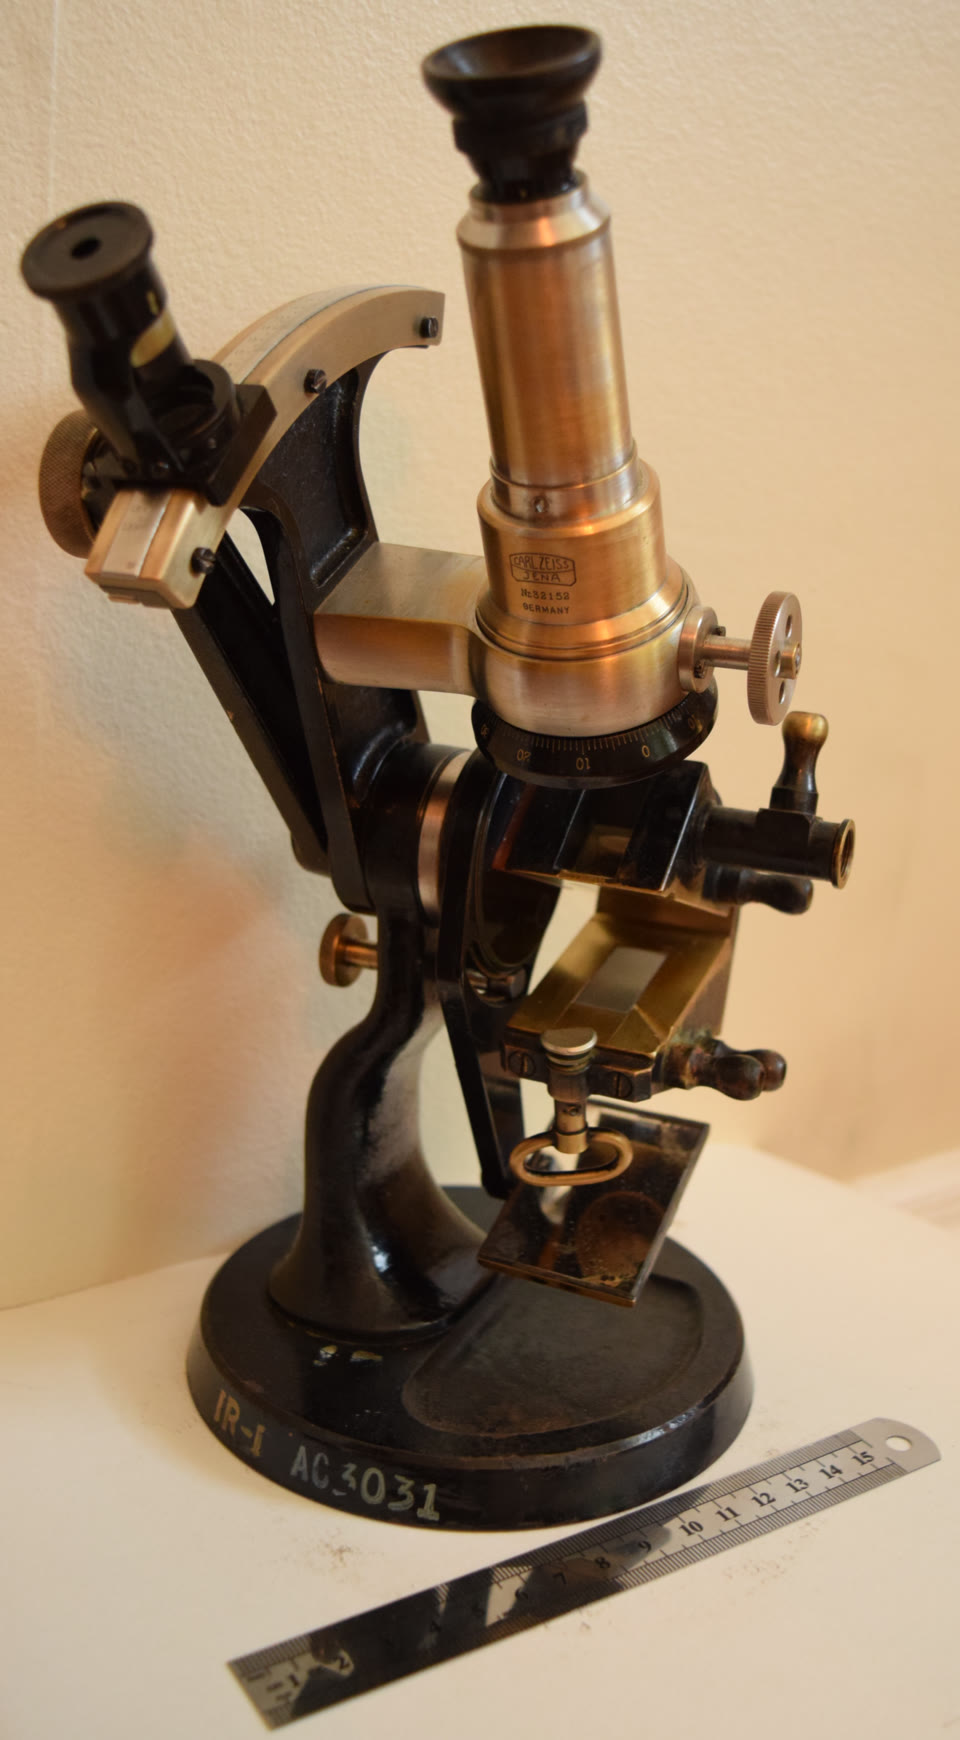
\includegraphics[height=6cm]{images/book2/abbe-refractometer.jpg}

{\small एक ऐबे अपवर्तनमापी: द्रव की एक बूँद दो
प्रिज़्मों के बीच फैलाई जाती है; नेत्रिका आधा प्रकाशित और आधा अँधेरा क्षेत्र दिखाती है, और
सीमा को क्रॉस-तारों पर लाने पर पैमाने पर अपवर्तनांक मिल जाता है।
छायाचित्र: फ़ोरेड, CC BY-SA 4.0, विकिमीडिया कॉमन्स।}
\end{omfigure}

\section{अभ्यास}

\begin{exercise}[$\star$]\label{exo:b1:lab-techniques-1:1}
प्रोपेनोन की एक बोतल पर चित्रलेख GHS02 और GHS07 और
कथन H225, H319 और H336 हैं। उस पर कौन-सा \omterm{def:b1:lab-techniques-1:ghs}{संकेत शब्द} है? कौन-से
कथन भौतिक \omterm{def:b1:lab-techniques-1:hazard}{संकट} का वर्णन करते हैं, कौन-से स्वास्थ्य संकट का? उनके द्वारा अपेक्षित दो
सावधानियाँ बताइए।
\end{exercise}

\begin{exercise}[$\star$]\label{exo:b1:lab-techniques-1:2}
\omterm{def:b1:lab-techniques-1:hazard}{संकट} या \omterm{def:b1:lab-techniques-1:hazard}{जोखिम}? (a) सांद्र सल्फ़्यूरिक अम्ल गंभीर जलन उत्पन्न करता है।
(b) धूम-कोष्ठ में दस्तानों के साथ किसी विषैले चूर्ण का \qty{50}{mg} तौलना
संचालक को थोड़ा ही अनावृत करता है। (c) सोडियम जल के साथ हाइड्रोजन मुक्त करता है।
(d) वही विलायक बंद बोतल में ठंडे की तुलना में खुले बीकर में गरम प्रयुक्त होने पर
अधिक ख़तरनाक है।
\end{exercise}

\begin{exercise}[$\star$]\label{exo:b1:lab-techniques-1:3}
किसी TLC प्लेट पर निक्षालक अग्र आधार-रेखा से \qty{6.0}{cm} ऊपर है;
नमूना \qty{2.1}{cm} और \qty{4.2}{cm} पर धब्बे देता है। उनके
$R_f$ परिकलित कीजिए। उसी प्लेट पर रखा गया एक संदर्भ \qty{4.2}{cm} तक चढ़ता है:
क्या निष्कर्ष निकाला जा सकता है और क्या नहीं?
\end{exercise}

\begin{exercise}[$\star$]\label{exo:b1:lab-techniques-1:4}
हर \qty{0.1}{mL} पर अंशांकित ब्यूरेट आधे भाग तक पढ़ी जाती है।
एक पठन की, फिर दो पठनों के अंतर के रूप में दिए गए
आयतन की \omterm{def:b1:lab-techniques-1:uncertainty}{मानक अनिश्चितता} परिकलित कीजिए।
\end{exercise}

\begin{exercise}[$\star\star$]\label{exo:b1:lab-techniques-1:5}
एक ही नमूने के पाँच तौल \qty{0.2512}{g}, \qty{0.2508}{g},
\qty{0.2515}{g}, \qty{0.2510}{g} और \qty{0.2505}{g} देते हैं। माध्य,
प्रायोगिक मानक विचलन, माध्य की \omterm{def:b1:lab-techniques-1:uncertainty}{मानक अनिश्चितता} परिकलित कीजिए,
और $k = 2$ के साथ परिणाम प्रस्तुत कीजिए।
\end{exercise}

\begin{exercise}[$\star\star$]\label{exo:b1:lab-techniques-1:6}
किसी कार्बनिक विलायक और जल के बीच \omterm{def:b1:lab-techniques-1:partition-coefficient}{विभाजन गुणांक} $K = 3$ वाले एक विलेय का
\qty{50}{mL} जल से कुल \qty{30}{mL} विलायक द्वारा निष्कर्षण किया जाता है।
एक भाग में, \qty{15}{mL} के दो भागों में,
और \qty{10}{mL} के तीन भागों में निष्कर्षित अंश परिकलित कीजिए।
\end{exercise}

\begin{exercise}[$\star\star$]\label{exo:b1:lab-techniques-1:7}
एक \omterm{def:b1:titration-methods:titration}{अनुमापन} \qty{0.1012}{mol/L} सांद्रता देता है, जिसकी \omterm{def:b1:lab-techniques-1:uncertainty}{मानक
अनिश्चितता} \qty{0.0006}{mol/L} है; विलयन
\qty{0.1000}{mol/L} पर बनाया गया था, जिसकी \omterm{def:b1:lab-techniques-1:uncertainty}{मानक अनिश्चितता} \qty{0.0002}{mol/L} है। क्या
दोनों मान संगत हैं? और यदि \omterm{def:b1:titration-methods:titration}{अनुमापन} की अनिश्चितता
\qty{0.0004}{mol/L} होती?
\end{exercise}

\begin{exercise}[$\star\star$]\label{exo:b1:lab-techniques-1:8}
तीन विलायकों में एक ठोस की \omterm{def:b1:precipitation:solubility}{विलेयताएँ} (उदाहरणार्थ मान, प्रति \qty{100}{mL} \unit{g}) ये हैं:
विलायक P, ठंडे में 1.5 और उबलते में 2.0; विलायक
Q, ठंडे में 0.3 और उबलते में 12; विलायक R, ठंडे में 9 और उबलते में 25। कौन-सा
विलायक \omterm{def:b1:lab-techniques-1:recrystallisation}{पुनःक्रिस्टलन} के लिए उपयुक्त है, और अन्य दो क्यों नहीं? सही
विलायक के साथ, यदि उबलते विलायक की न्यूनतम मात्रा प्रयुक्त हो और
मिश्रण ठंडा किया जाए, तो ठोस के \qty{5.0}{g} का अधिकतम कितना अंश पुनःप्राप्त हो सकता है?
\end{exercise}

\begin{exercise}[$\star\star$]\label{exo:b1:lab-techniques-1:9}
\qty{20}{\celsius} पर ताप-स्थिर किए गए एक रंगहीन द्रव का
$n_D = 1.3612$ है। वह जल, एथेनॉल और साइक्लोहेक्सेन में से कौन-सा हो सकता है? ताप
क्यों बताया जाता है? 1.350 का मान क्या सुझाता?
\end{exercise}

\begin{exercise}[$\star\star\star$]\label{exo:b1:lab-techniques-1:10}
\cref{exo:b1:lab-techniques-1:6} के आँकड़ों के साथ दिखाइए कि
\qty{30}{mL} विलायक को चाहे कितने भी सूक्ष्म भागों में बाँटा जाए, विलेय का अधिक से अधिक
$1 - \mathrm{e}^{-KV/V_a}$ अंश निष्कर्षित किया जा सकता है, और उसे परिकलित कीजिए।
उस सीमा के \qty{99}{\percent} तक कितने भाग पहुँचते हैं?
\end{exercise}

\begin{exercise}[$\star\star\star$]\label{exo:b1:lab-techniques-1:11}
एक राशि के बारे में ज्ञात है कि वह $x_0 - a$ और $x_0 + a$ के बीच है, और
$x_0$ के निकट के मान अधिक संभाव्य हैं: उसका घनत्व त्रिभुजाकार है, $(a - |x - x_0|)/a^2$।
जाँचिए कि वह प्रसामान्यीकृत है और दिखाइए कि उसकी \omterm{def:b1:lab-techniques-1:uncertainty}{मानक अनिश्चितता}
$a/\sqrt6$ है। आयताकार स्थिति से तुलना कीजिए।
\end{exercise}

\begin{exercise}[$\star\star\star$]\label{exo:b1:lab-techniques-1:12}
\cref{exo:b1:lab-techniques-1:5} के नमूने (मोलर द्रव्यमान \qty{204.2}{g/mol}, उसकी
अनिश्चितता नगण्य) को \qty{100.00}{mL} के आयतनमितीय फ़्लास्क में घोलकर एक मानक विलयन
बनाया जाता है, जिसके आयतन की \omterm{def:b1:lab-techniques-1:uncertainty}{मानक अनिश्चितता} \qty{0.06}{mL} है।
सांद्रता और उसकी आपेक्षिक तथा \omterm{def:b1:lab-techniques-1:uncertainty}{विस्तारित अनिश्चितताएँ} परिकलित कीजिए। कौन-सा
स्रोत प्रभावी है?
\end{exercise}

\section{समस्या: ऐस्पिरिन का शोधन}

\begin{problem}[{सप्ताहांत समस्या --- एक संश्लेषण के संकट,
अपरिष्कृत ऐस्पिरिन का पुनःक्रिस्टलन और उसकी लब्धि, A-प्रकार और B-प्रकार
अनिश्चितताओं के साथ एक गलनांक, और सारणीबद्ध मान से
प्रसामान्यीकृत विचलन}]
\label{pb:b1:lab-techniques-1:1}
एक विद्यार्थी \qty{2.00}{g} सैलिसिलिक अम्ल को एथेनोइक ऐनहाइड्राइड के
आधिक्य के साथ गरम करके ऐस्पिरिन बनाता है, फिर अपरिष्कृत उत्पाद का \omterm{def:b1:lab-techniques-1:recrystallisation}{पुनःक्रिस्टलन} करता है।
मोलर द्रव्यमान (\unit{g/mol}): सैलिसिलिक अम्ल \ce{C7H6O3} 138.0, ऐस्पिरिन
\ce{C9H8O4} 180.0, एथेनोइक ऐनहाइड्राइड \ce{C4H6O3} 102.0। लेबल:
सैलिसिलिक अम्ल GHS05, GHS07, H302, H318; एथेनोइक ऐनहाइड्राइड GHS02,
GHS05, GHS06, GHS07, H226, H302, H314, H332; ऐस्पिरिन GHS07, H302।
जल में ऐस्पिरिन की \omterm{def:b1:precipitation:solubility}{विलेयता}: \qty{25}{\celsius} पर \qty{3.3}{g/L}।
ऐस्पिरिन का सारणीबद्ध गलनांक (तीव्र तापन): \qty{135}{\celsius}।
% ledger: ghs:salicylic, ghs:acetic-anhydride, ghs:aspirin, sol:aspirin-25,
% mp:aspirin, hstat:H318, hstat:H226, hstat:H314, hstat:H302

\medskip
\noindent\textbf{भाग I --- \omterm{def:b1:lab-techniques-1:hazard}{संकट}।}
\begin{enumerate}
  \item एथेनोइक ऐनहाइड्राइड के लेबल का हर चित्रलेख क्या अर्थ रखता है?
  \item सैलिसिलिक अम्ल के लेबल पर कौन-सा \omterm{def:b1:lab-techniques-1:ghs}{संकेत शब्द} है? और
        ऐस्पिरिन के लेबल पर?
  \item एथेनोइक ऐनहाइड्राइड के \omterm{def:b1:lab-techniques-1:hazard}{संकट} अधिक गंभीर हैं। समझाइए कि
        उसके \qty{5}{mL} को संभालने का \omterm{def:b1:lab-techniques-1:hazard}{जोखिम} फिर भी कैसे छोटा किया जा सकता है।
  \item ऐनहाइड्राइड के कौन-से कथन चश्मे और दस्तानों की माँग करते हैं,
        और कौन-से धूम-कोष्ठ और लौ की अनुपस्थिति की?
  \item यदि ऐनहाइड्राइड की एक बूँद आँख में पहुँच जाए तो तुरंत क्या किया जाता है?
  \item \omterm{def:b1:lab-techniques-1:recrystallisation}{पुनःक्रिस्टलन} के निस्यंद में जल में एथेनोइक अम्ल और थोड़ा
        एथेनॉल है। वह कहाँ जाता है?
\end{enumerate}

\noindent\textbf{भाग II --- संश्लेषण और \omterm{def:b1:lab-techniques-1:recrystallisation}{पुनःक्रिस्टलन}।}
\begin{enumerate}[resume]
  \item उपोत्पाद के रूप में एथेनोइक अम्ल
        \ce{C2H4O2} के साथ संश्लेषण का समीकरण लिखिए, और जाँचिए कि वह संतुलित है।
  \item सैलिसिलिक अम्ल की मात्रा और ऐस्पिरिन का अधिकतम द्रव्यमान
        परिकलित कीजिए।
  \item अपरिष्कृत शुष्क उत्पाद का भार \qty{2.41}{g} है। यह
        अधिकतम का \qty{92}{\percent} होने पर भी \omterm{def:b1:lab-techniques-1:recrystallisation}{पुनःक्रिस्टलन} को
        छोड़ा क्यों नहीं जा सकता?
  \item ऐस्पिरिन का \omterm{def:b1:lab-techniques-1:recrystallisation}{पुनःक्रिस्टलन} थोड़े एथेनॉल में गरम जल मिलाकर
        किया जाता है। क्वथनांक के पास की \omterm{def:b1:precipitation:solubility}{विलेयता} की तुलना में \qty{25}{\celsius} पर जल में
        \omterm{def:b1:precipitation:solubility}{विलेयता} ही वह गुण क्यों है जो मायने रखता है?
  \item अपरिष्कृत ठोस को गरम विलायक की न्यूनतम मात्रा में क्यों घोला जाता है?
  \item विलयन को धीरे-धीरे, फिर बर्फ़ में, क्यों ठंडा किया जाता है?
  \item \qty{25}{\celsius} पर \qty{40}{mL} निस्यंद कीप से निकलता है,
        फिर \qty{5}{mL} धोवन जल। उनके साथ खोई ऐस्पिरिन के
        द्रव्यमान का आकलन कीजिए।
  \item शुद्ध शुष्क उत्पाद का भार \qty{1.95}{g} है। \omterm{def:b1:extent-q-and-k:fractional-extent}{लब्धि} परिकलित कीजिए।
\end{enumerate}

\noindent\textbf{भाग III --- गलनांक।}
\begin{enumerate}[resume]
  \item ठीक पहले अंशशोधित बेंच पर छह पठन 134, 135,
        133, 135, 134 और \qty{136}{\celsius} देते हैं। माध्य परिकलित कीजिए।
  \item प्रायोगिक मानक विचलन परिकलित कीजिए।
  \item माध्य की A-प्रकार \omterm{def:b1:lab-techniques-1:uncertainty}{मानक अनिश्चितता} निकालिए।
  \item हर पठन निकटतम डिग्री तक लिया गया है। पठन की B-प्रकार
        अनिश्चितता परिकलित कीजिए।
  \item बेंच का अंशशोधन $\pm\qty{1}{\celsius}$ के भीतर
        प्रत्याभूत है। संगत B-प्रकार
        अनिश्चितता परिकलित कीजिए, फिर संयुक्त \omterm{def:b1:lab-techniques-1:uncertainty}{मानक अनिश्चितता}।
  \item गलनांक को उसकी \omterm{def:b1:lab-techniques-1:uncertainty}{विस्तारित अनिश्चितता} ($k = 2$) के साथ प्रस्तुत कीजिए।
  \item एक सहपाठी का अपरिष्कृत उत्पाद 120 और
        \qty{128}{\celsius} के बीच पिघलता है। यह क्या दर्शाता है?
\end{enumerate}

\noindent\textbf{भाग IV --- संदर्भ से तुलना।}
\begin{enumerate}[resume]
  \item सारणीबद्ध मान इकाई तक दिया गया है। इससे कौन-सी \omterm{def:b1:lab-techniques-1:uncertainty}{मानक
        अनिश्चितता} निहित है?
  \item किसी TLC प्लेट पर (अग्र \qty{6.0}{cm}) अपरिष्कृत उत्पाद
        \qty{2.3}{cm} और \qty{3.3}{cm} पर धब्बे दर्शाता है, सैलिसिलिक अम्ल
        \qty{2.3}{cm} पर एक धब्बा, पुनःक्रिस्टलित उत्पाद
        \qty{3.3}{cm} पर एक धब्बा। $R_f$ मान परिकलित कीजिए और निष्कर्ष निकालिए।
  \item ऐस्पिरिन का गलनांक तापन दर पर क्यों निर्भर करता है?
  \item मापे गए और
        सारणीबद्ध गलनांकों के बीच \omterm{def:b1:lab-techniques-1:z-score}{प्रसामान्यीकृत विचलन} $z$ परिकलित कीजिए, और बताइए कि वे संगत हैं या नहीं।
\end{enumerate}
\end{problem}
